\documentclass{article}
\usepackage[utf8]{inputenc}
\usepackage{url}
\usepackage{graphicx}
\graphicspath{ {./images/} }
\usepackage{pdfpages}
\usepackage{booktabs}
\usepackage{xcolor,colortbl}
\usepackage{geometry}
\geometry{
 a4paper,
 total={170mm,257mm},
 left=20mm,
 top=20mm,
}

\usepackage{caption}
\usepackage{subcaption}

\usepackage{fullpage}
\usepackage{times}
\usepackage{fancyhdr,graphicx,amsmath,amssymb}
\usepackage[ruled,vlined]{algorithm2e}

%%%%%%%%%%%%%%%%%%%%%%%%%%%%%%%%%%%%%%%%%%%%%%%%%%

\title{Weekly Log}
\author{Luke Kurlandski}

\begin{document}

\maketitle

%%%%%%%%%%%%%%%%%%%%%%%%%%%%%%%%%%%%%%%%%%%%%%%%%%

\section*{W1: 08/21/2022}

\subsection*{Notes}

\begin{itemize}
\item There are limited examples of applying LMs specifically to malware. Found no examples of using a highly advanced transformer-based architecture, such as BERT.
\item Could possibly train a code LM specifically on malware, e.g., MalBERT or MalELECTRA.
\item Malware generation using seq2seq? Malware obfuscation using code-repair techniques?
\item Several works use word2vec, RNNs, LSTMs for language modeling malware, but there is no one paper that uses all three on the same dataset for a holistic comparison. Furthermore, most of these datasets are not publicly available.
\item No paper has used the AST approach taken by Uri Alon et al. specifially for malware
\item Perhaps use a large language model of code after decomposition, such as PolyCoder, for the classification? Or would this not work because the decompiled malware would not have useful identifiers? Would it work if ASTs were used to train the LM?
\item Is there a BERT for Assembly language? If so, that could be an excellent LM for malware.
\end{itemize}

\subsection*{Report}

\begin{itemize}
\item Reading about malware detection and classification
\item At this point I'm probably more comfortable/qualified with static malware detection than dynamic detection
\item The research in using language modeling techniques on malware is fairly new and undeveloped
\item Many papers doing this do not compare their methods to any baseline method
\item Many do not use publicly available datasets
\item Ideal dataset for this research is probably Sophos-ReversingLabs 20 Million dataset
\end{itemize}

\subsection*{Minutes}

\begin{itemize}
\item This week I will work on replicating some of the experimental results produced in other papers
\end{itemize}

\pagebreak

%%%%%%%%%%%%%%%%%%%%%%%%%%%%%%%%%%%%%%%%%%%%%%%%%%

\section*{W2: 08/27/22}

\subsection*{Onboarding Meeting}

\begin{itemize}
	\item Dr. Pan, Dr. Wright, and I will meet during the Malware Group meeting time, during the reading group when I am presenting, and as needed.
	\item The RPA is essentially a short research paper with a robust literature review. 
	\item I should begin preparation for it immediately. 
	\begin{itemize}
		\item See rubrics on RIT site.
		\item Could focus on a particular type of malware detection, such as Windows macro malware, PDF malware or more general malware detection.
		\item Could look into generating adversarial malware examples, along the lines of code2vec.
	\end{itemize}
	\item ``binary lifting'' from binary to intermediate (similar to assembly, which could be recompiled again)
	\item Goal is for second half of semester to have a solid objective for research
	\item Innovation: if its been done ten times, its not innovative enough
	\item Read other students' RPAs
\end{itemize}

\subsection*{Notes}

\begin{itemize}
	\item Adversarial malware: generate embeddings for malware opcode and substitute to fool the detector
	\item Little research done on poisoning attacks
\end{itemize}

\subsection*{Report}

\begin{itemize}
	\item Read about adversarial malware generation and defense.
	\item Most literature is concerned with adapting CV methods that use continuous representations to malware with discrete representations.
	\item Might be novel to explore adversarial malware with continuous representations, i.e., malware represented using a learned embedding.
	\item Adversarially modifying the embedding would be simple, but figuring out how that can be achieved by modifying the malware itself would be challenging.
	\item Look into NLP/CV/audio processing adversarial techniques that use embeddings.
	\item Dr. Pan suggested and idea of swapping malware API calls with similar calls as an adversarial approach.
	\item If using embeddings as a feature representation this would fit into that idea nicely.
\end{itemize}

\subsection*{Minutes}

\begin{itemize}
	\item Develop a plan for the semester
\end{itemize}

\pagebreak

%%%%%%%%%%%%%%%%%%%%%%%%%%%%%%%%%%%%%%%%%%%%%%%%%%

\section*{W3: 09/02/2022}

\subsection*{Notes}

\begin{itemize}
	\item Would using LM techniques in malware detection make them robust to adversarial attacks?
	\item Idea: build a [novel?] LM-based classifier, demonstrate its robustness to adversarial attacks, propose a new adversarial attack based upon NLP techniques!!!! Preferably use windows, android, and PDF datasets
	\item AST for assembly code probably not logical, but would it even be needed?
	\item Diverse ensembles more robust to adversarial attacks?
	\item Could be interesting to train an ensemble using dramatically different feature reps, then test an RL, GAN, Graph, and traditional Adversarial malware attacks
	\item Research on attacks should be focused on the black box problem space scenario.
	\item Identify problematic sequences of opcode and replace them with computationally equivalent ones to fool detector?
	\item Adversarial Malware needs to be verified for correctness in Cuckoo Sandbox
	\item An adversarial attack designed specifically for ensembles?
	\item Adversarial training works...but is there a point where retraining fails?
	\item Have RL, genetic, or GAN attacks been tested against ensembles? One paper tested various attacks against a small ensemble, but what about a large one? IE test black box attacks against ensembles, possibly that use different feature reps.
	\item Test ensembles using different feature rep vs ensembles using the same feature rep
	\item Read every source that uses black box attacks in the feature space. Determine whether or not their methods use reasonable defense mechanisms. Test their methods using reasonable defense mechanisms.
	\item Does the surrogate model negate the black box model entirely? Are all black box attacks really white box?
	\item Testing adversarial techniques against AV software would be more practical than just testing against a single DNN
	\item Idea: adversarial testing against an ensemble of AV softwares, like VirusTotal
\end{itemize}

\subsection*{Report}

\begin{itemize}
	\item Read more about adversarial malware evasion attacks
	\item Observed that many attacks assume unrealistic knowledge about the classification system or are ineffective at or incapable of producing functioning adversarial examples
	\item Existing black box, practical adversarial evasion attacks generally use ``easy'' classifiers
	\item Interesting to see how their techniques hold up against a more realistic defender, like an ensemble or a commercial AV product
\end{itemize}

\subsection*{Minutes}

\begin{itemize}
	\item 
\end{itemize}

\pagebreak

\section*{W4: 09/12/22 - 09/19/22}

%%%%%%%%%%%%%%%%%%%%%%%%%%%%%%%%%%%%%%%%%%%%%%%%%%

\subsection*{General}
\begin{itemize}
	\item Concerning swapping blocks of suspicious code with less suspicious but equivalent alternatives, the AST approach might be useful because it represents the actual functionality of the code and code produce code that functions the same, but uses weird sequences of tokens.
	\item Could use code2seq to take assembly to language, then use codex to take language to assembly to get non deterministic outputs
	\item Interesting paper that uses trains GPT2 on malware bytecode
	\item Perhaps a code generation tool like codex could repeatedly nondeterministically mask and substitute chunks of assembly for adversarial evasion
	\item Use codex to modify the source code of malware
	\item Large scale ``instruction substitution'' in poisoning attacks?
	\item Using code generation techniques to change the important code itself is an extremely challenging problem. Several methods use various strategies to append some form of bytes into sections of the code. We could use code generation techniques to insert logically functional code blocks into the malware. At that point though, we might as well just copy and paste assembly from a specific source. 
	\item Could use code generation to write C code, then compile it, and insert the compiled code into the malware. Use genetic or RL algorithms to find where to insert it, or simply insert it behind a if-false statement.
	\item Code summarization of a portion of assembly code via code2vec or something like it. Then code generation from the summary back into assembly.
	\item To create a labeled assembly language, compile C code and use function names as labels.
	\item Shellcode\_IA32 has some code generation with codeBERT
	\item PalmTree is a really effective embedding setup
	\item Potentially use the function boundary identification to identify functions to swap
	\item Perform seq2seq learning trying to make the frequency of opcodes match that of goodware. Evaluate upon unit tests for C code.
\end{itemize}

\subsection*{Malware Group}
\subsubsection*{Report}
\begin{itemize}
	\item Interested in Adversarial Malware Evasion Attacks
\end{itemize}
\subsubsection*{Minutes}
\begin{itemize}
	\item Code generation techniques to produce adversarial examples, eg, code2vec/code2seq on assembly
	\item Would have to generate code that functions, but doesn't appear malicious.
	\item Oakland paper Saidur shared in the Slack group
	\item Android research might be more promising than PE research
	\item Benign Android data is easier to attain
	\item AndroidZoo is a widely used dataset
	\item Dr. Pan will send out some papers
\end{itemize}

\subsection*{Reading Group}
\begin{itemize}
	\item 
\end{itemize}

\subsection*{Weekly Scrum}
\subsubsection*{Report}
\begin{itemize}
	\item Looking into using LLMs for adversarial malware generation
	\item Hard problem and not exactly sure what directions to focus on
	\item The start would be with a language model at the assembly or binary level
	\item The state-of-the-art seems to be PalmTree (Pre-trained Assembly Language Model for InsTRuction EmbEdding), which uses a BERT architecture with different training tasks adopted for code
	\item This gives us really good embeddings for assembly instructions
	\item BERT has been adopted for sequence tasks in natural language and in code tooling, so there could be some extensions made to PalmTree to get interesting things going at the assembly level
	\item Took a little bit of wandering to find PalmTree and other binary analysis tools
	\item This weekend, will develop more concrete ideas and write up that abstract
\end{itemize}
\subsubsection*{Minutes}
\begin{itemize}
	\item Injecting code underneath if false blocks probably not a good direction to take
	\item Probably need to perform some kind of function segmentation
\end{itemize}

\pagebreak

\section*{W5: 09/19/22 - 09/26/22}

%%%%%%%%%%%%%%%%%%%%%%%%%%%%%%%%%%%%%%%%%%%%%%%%%%

\subsection*{General}
\begin{itemize}
	\item Dr. Wright has mentioned modifying API calls...wouldn't this have to be done at the source code level? I let my knowledge of Operating Systems and Computer Architecture fade a little...
	\item Using code2code to modify the byte histograms and byte-entropy of EMBER might be successful
	\item Explainability of EMBER
	\item Microsoft Malware Classification Challenge (MMCC) is a multiclass classification challenge. This could be an alternative to benign/malicious classification because it alleviates the challenges associated with gathering benign data.
	\item Function identification at the assembly level to build monolingual corpora
\end{itemize}

\subsection*{Malware Group}
\subsubsection*{Report}
\begin{itemize}
	\item Worked out a research objective for the remainder of the semester
	\item Wright/Pan talked about replacing suspicious sections of code as part of an adversarial attack
	\item Should be able to use sequence to sequence models, similar to machine translation or transcompilation
	\item Related work:
	\begin{itemize}
		\item LLM for assembly code prior to fine-tuning for downstream tasks
		\item Generating assembly-level code from English descriptions
	\end{itemize}
	\item I think we can use a pre-trained LLM encoder-decoder architecture to perform the translation
	\item Things that remain to be worked out are:
	\begin{itemize}
		\item What makes assembly code look suspicious vs benign?
		\item How to actually train the model, eg supervised/unsupervised and what is the objective?
	\end{itemize}
	\item What I need to do:
	\begin{itemize}
		\item Learn more about sequence to sequence models, neural machine translation, and transcompilation
		\item Learn more about the properties of malware vs benignware
	\end{itemize}
	\item Other:
	\begin{itemize}
		\item Produce abstract from these ideas
		\item Presentation tomorrow remotely
	\end{itemize}
\end{itemize}
\subsubsection*{Minutes}
\begin{itemize}
	\item Features of malicious code: 
	\item Look at sequence of API calls. Here's what we see in ransom ware. Could just start opening up other files in the API calls. Default approach:  run a model on the malware and figure out what is important. Or use gradient based methods to figure out what is important. 
	\item Statically we know what API calls are imported and control flow graphs. Dynamically we can get the sequence of API calls. 
	\item Histogram of byte sequence frequencies
	\item Substitute API calls
	\item Find API calls that can be substituted
	\item Identify certain functions/areas that are malicious looking
	\item Could use histogram/heat map to identify those regions
	\item Gadgets: 
	\item \textbf{using explainability, figure out what are chunks of code flagged for maliciousness, then construct a number of replacement sequences. Dumb version is to just generate some kind of replacement and test to see if it works. Smart version is to replace bit by bit and monitor the gradient of the loss function. Then follow the loss function greedily. }
	\item Maybe don't worry about making the malware runable
	\item Identify code and replace with code that has the same functionality
	\item \textbf{One identify the functions to be changed by explainable. This by itself could be a very interesting problem. See if this has already been done. } 
	\item Saidur will share some papers about histograms
\end{itemize}

\subsection*{Reading Group}
\begin{itemize}
	\item Yin Pan complemented my presentation skills
	\item Could have been better prepared for some of the results sections
	\item Could have worked out a method of having a few notes
\end{itemize}

\subsection*{Weekly Scrum}
\subsubsection*{Report}
\begin{itemize}
	\item Looked into using explainability to decide which regions of malware code could be modified
	\item Started with EMBER classifier
	\begin{itemize}
		\item Can precisely determine the importance of all features used by the GBT model
		\item Saidur's discussed using byte histograms as a classification feature
		\item Between 7\%-12\% of EMBER's decision making process can be attributed to these features
		\item Simply manipulating these properties could work on EMBER
	\end{itemize}
	\item Byte-stream classifiers (MalConv)
	\begin{itemize}
		\item A few papers investigate methods to observe, which portions of the malware trigger high gradient activation, ie, they are important
		\item Regions of high activation seem to be distributed throughout the malware file, which means that an attack made only to the code could still be effective
		\item Next paper on my plate uses explainability of MalConv as part of an attack
	\end{itemize}
	\item Dr. Wright brought up some ideas about API calls...wouldn't those modifications need to be performed at the source code level? 
	\item I find this term API call rather nebulous...could you give a specific example
\end{itemize}
\subsubsection*{Minutes}
\begin{itemize}
	\item 
\end{itemize}

\subsection*{Malware Group}
\subsubsection*{Report}
\begin{itemize}
	\item Code Generation Attack
	\begin{itemize}
		\item Related work to determine which regions within malware MalConv learns the most from
		\item Sources differ on whether gradient activation is highest within headers
		\item Unknown why classifier identifies the regions, which could help generate benign-looking code
		\item Alternatively, could turn to machine translation techniques
		\begin{itemize}
			\item Frame problem as have source and target languages
			\item Source language is malicious-looking code; target is benign-looking code
			\item Use unsupervised NMT methods that require no parallel data
			\item Denoising Auto Encoder: reconstruct source from noisy source input
			\item Backtranslation: use source-to-target and target-to-source models trained in unison (similar to GANs)
			\item Inspired by Backtranslation: On the Fly Back Translation, Cross Domain Training
			\item Summarize and Generate: source code to NL, NL to target code
		\end{itemize}
		\item MT is generally considered a simpler task than generation, so this might be helpful approach
		\item Wouldn't Dr. Wright's discussion of API calls need to take place at the level of source code?
	\end{itemize}
	\item After reading many papers analyzing MalConv, I started thinking about how it could be improved
	\item Enhancing MalConv
	\begin{itemize}
		\item Went on a tangent for the past several days
		\item MalConv learns an 8 dimensional embedding layer during training
		\item Interested in using pretrained embedding layer
		\item Train MalConv-like classifier on assembly instead of raw bytes
		\item Maintains the spirit of MalConv
		\item Major performance enhancements made to MalConv in 2021 improve memory usage and training time
		\item Pretrained embeddings could yield a higher performing MalConv with less training data
		\item Idea is less novel, but more concrete
	\end{itemize}
\end{itemize}
\subsubsection*{Minutes}
\begin{itemize}
	\item Look into how to do this stuff with Android
	\item Yin will send a paper on obfuscation Android stuff
	\item Wright is not interested in using pretrained embeddings in malware detection
	\item Old student built something that moved from machine code to IR to machine code
	\item Potentially incorporate some of the automatic unit testing stuff
	\item Will have a discussion with Dr. Wright on Tuesday/Thursday
\end{itemize}

\pagebreak

%%%%%%%%%%%%%%%%%%%%%%%%%%%%%%%%%%%%%%%%%%%%%%%%%%

\section*{Week 6}
11:00 Monday 09/26/22 - 10:59 Monday 10/03/22

\subsection*{General}
\begin{itemize}
	\item Which citation should I grab when multiple citations exist?
\end{itemize}

\subsection*{Reading Group}
\begin{itemize}
	\item Canceled
\end{itemize}

\subsection*{One on One with Dr. Wright}
\begin{itemize}
	\item Unit Test Creation
	\begin{itemize}
		\item Could manually make unit tests for a number of malicious chunks of code
		\item Look into possible automatic unit testing frameworks for assembly
		\item Then when swapping them with benign-looking variants, could test to verify that they work
		\item The hope would be that the malicious-looking chunks are a feature of many malware samples, so the unit test creation would not have to be repeated
	\end{itemize}
	\item Unit Test Mapping
	\begin{itemize}
		\item Could also use open source code with available unit tests
		\item build embeddings for chunks of code in malware
		\item Find unit-tested code that has the same embedding!
	\end{itemize}
\end{itemize}

\subsection*{Weekly Scrum}
\subsubsection*{Report}
\begin{itemize}
	\item 
\end{itemize}
\subsubsection*{Minutes}
\begin{itemize}
	\item 
\end{itemize}

\subsection*{Malware Group}
\subsubsection*{Report}
\begin{itemize}
	\item Working on building non-parallel monolingual corpora for translation approach
	\item My skills in Pytorch are somewhere in between novice and intermediate
	\item Burned a lot of time making little progress due to stupid hangups, eg, beta versions of Captum, torchtext, torchvision, ambiguous documentation of third part dependencies, bugs in research codebases
	\item Where I stand right now:
	\begin{itemize}
		\item Have functioning pretrained CNN classifier
		\item Have SOREL-20M PE Malware dataset
	\end{itemize}
	\item What I'm working on
	\begin{itemize}
		\item Figuring out how to use Captum explainability 
	\end{itemize}
\end{itemize}
\subsubsection*{Minutes}
\begin{itemize}
	\item We need some sort of proof-of-concept that the translation is possible 
	\item Malware authors modify the code in extremely bizarre ways to fool malware analysts
	\item Try to find some example of obfuscated malware that triggers a classifier; substitute it with code that makes the classifier less confident
	\item For RPA
	\begin{itemize}
		\item Clear understanding of the literature
		\item Understanding of how to advance the state of the art
		\item Preliminary results
	\end{itemize}
\end{itemize}

\pagebreak

%%%%%%%%%%%%%%%%%%%%%%%%%%%%%%%%%%%%%%%%%%%%%%%%%%

\section*{Week 7 \& 8}
11:00 Monday 10/03/2022 - 10:59 Monday 10/10/2022

\subsection*{General}
\begin{itemize}
	\item 
\end{itemize}

\subsection*{Reading Group (Tuesday)}
\begin{itemize}
	\item 
\end{itemize}

\subsection*{Weekly Scrum (Thursday)}
\subsubsection*{Report}
\begin{itemize}
	\item Need to demonstrate that we can rewrite pieces of malware to make them look less like malicious
	\item To do this, I plan to measure the importance of a chunk of code, rewrite it, and then remeasure it
	\item Goes back to using explainability to find malicious looking chunks of code, which has not gone smoothly
	\item Selected LowMemMalConv/MalConvGCT because I have pretrained models
	\item Spent several trying to apply integrated gradients, which I now believe is not possible
	\item Can work around the embedding layer, but MalConv2 has other complex non-differentiable layers
	\item Working on perturbation-based explainability methods, eg Feature Ablation, Shapley Value Sampling
	\item Complexity has a linear relationship to the number of features, which for the raw-byte classifiers is large
	\item Plan on running that code over the weekend, hopefully over an ssh connection from New Jersey
	\item May want to write and train a simple raw-byte classifier soon so I can use the gradient methods
	\item This brings up challenges associated with acquiring benign training
\end{itemize}
\subsubsection*{Minutes}
\begin{itemize}
	\item 
\end{itemize}

\subsection*{Malware Group (Monday)}
\subsubsection*{Report}
\begin{itemize}
	\item Have results of several explainability experiments on eight malicious/benign executables
	\begin{itemize}
		\item Feature Perturbation
		\item Feature Occlusion
		\item Occlusion
		\item Shapley Value Sampling
	\end{itemize}
	\item Have file offset positions of highly relevant regions of malware
	\item Working with IDA to modify them
	\item Dr. Pan has mentioned ASTs a few times. At the moment, I'm keeping structured representations of code in mind for later stages of my project, unless you think they would be extremely useful at this moment?
	\item Have access to AndroZoo dataset.
	\item Working on analyzing executables with Cuckoo Sandbox prior to modifying. Is this still the state of the art software for this task? Cuckoo 2.x only supports Python 2.7 at the moment, but a full rewrite is in the works to a Cuckoo 3.x series.
\end{itemize}
\subsubsection*{Minutes}
\begin{itemize}
	\item 
\end{itemize}

\pagebreak

%%%%%%%%%%%%%%%%%%%%%%%%%%%%%%%%%%%%%%%%%%%%%%%%%%

\section*{Week 9}
11:00 Monday 10/17/2022 - 10:59 Monday 10/24/2022

\subsection*{General}
\begin{itemize}
	\item partway through cuckoo sandbox setup
	\item left off at Preparing the Host > Configuration
\end{itemize}

\subsection*{Reading Group (Tuesday)}
\begin{itemize}
	\item Machine Unlearning, Saidur presentation
\end{itemize}

\subsection*{Weekly Scrum (Thursday)}
\subsubsection*{Report}
\begin{itemize}
	\item Canceled
\end{itemize}
\subsubsection*{Minutes}
\begin{itemize}
	\item 
\end{itemize}

\subsection*{Malware Group (Monday)}
\subsubsection*{Report}
\begin{itemize}
	\item Previously was working on producing a proof of concept example demonstrating that malware portions could be rewritten to reduce how suspicious they look
	\item Ended up getting sidetracked from that objective and I went ahead and produced nonparallel corpora of malicious-looking and benign-looking code snippets
	\item Several weeks ago I think I misspoke in one of our Thursday meetings about SHAP, differentiability, and MalConv; I used SHAP values to identify the malicious and benign regions of malware
	\item Started working on a sequence to sequence model to ingest x86 instructions and regurgitate x86 instructions
	\item Goal would be to build this up into an unsupervised translation model
	\item Had a slightly confusing email chain with Dr. Pan, could you clarify what you mean by workable malware?
\end{itemize}
\subsubsection*{Minutes}
\begin{itemize}
	\item 
\end{itemize}

\pagebreak

%%%%%%%%%%%%%%%%%%%%%%%%%%%%%%%%%%%%%%%%%%%%%%%%%%

\section*{Week 10}
11:00 Monday 10/24/2022 - 10:59 Monday 10/31/2022

\subsection*{General}
\begin{itemize}
	\item 
\end{itemize}

\subsection*{Reading Group (Tuesday)}
\begin{itemize}
	\item 
\end{itemize}

\subsection*{Weekly Scrum (Thursday)}
\subsubsection*{Report}
\begin{itemize}
	\item Trying to modify malware's .text section to flip classifier's prediction
	\item Tried substituting with 
	\begin{itemize}
		\item random bytes
		\item padding value
		\item benign-looking bytes from the same executable
		\item a benign executeable's entire .text section
	\end{itemize}
	\item These changes have caused only minor reduction in the classifier's confidence, e.g., .9999 to .9990
	\item Possible issues include
	\begin{itemize}
		\item Model hugely over confident
		\item Model trained on small collection of data and non-diverse benign data
		\item Using only first 1MB of the malware to make everything run faster
		\item Modifications made to processed input tensors instead of the raw binary
		\item Explainability methods not working well due to complexity of model
	\end{itemize}
	\item TODO:
	\begin{itemize}
		\item Carefully analyze my code for sources of error
		\item Perform the modifications in the file space instead of the feature space
		\item Reevaluate the importance of the different sections of the malware file
		\item Consider training a simpler CNN model, using a more complete dataset, or using entire malware file
	\end{itemize}
	\item Tool to open up a PE executable in an IDE-like environment and start typing x86 instructions?
\end{itemize}
\subsubsection*{Minutes}
\begin{itemize}
	\item 
\end{itemize}

\subsection*{Malware Group (Monday)}
\subsubsection*{Report}
\begin{itemize}
	\item Sequence to sequence model spits out x86 instructions (progress on boilerplate NLP, e.g., tokenization)
\end{itemize}
\subsubsection*{Minutes}
\begin{itemize}
	\item 
\end{itemize}

\pagebreak

%%%%%%%%%%%%%%%%%%%%%%%%%%%%%%%%%%%%%%%%%%%%%%%%%%

\section*{Week 11}
11:00 Monday 10/31/2022 - 10:59 Monday 11/06/2022

\subsection*{General}
\begin{itemize}
	\item Idea: clustering malware based upon PalmTree embeddings for classification
\end{itemize}

\subsection*{Report}
\begin{itemize}
	\item I am identifying the .text section location correctly.
	\item Issues still exist with certain files that may have been packed.
	\item For now I'm simply avoiding those files.
	\item Reason was not able to reduce classifier uncertainty in previous reports was that the benign executable I was performing swaps with was actually a false positive, so its .text section was malicious-looking.
	\item Experiment:
	\begin{itemize}
		\item 1424 true positive malware test files
		\item Record initial classifier confidences
		\item Substitute .text section with benign executable
		\item Mean reduction in confidence was 49\%
		\item Able to flip the prediction on 48\% of malware files
	\end{itemize}
\end{itemize}

\subsection*{Minutes}
\begin{itemize}
	\item Proof on concept demonstrated sufficiently
	\item Could test on multiple malware files or use the other MalConv classifier
\end{itemize}

\pagebreak

\subsection*{Supplementary Material}

Experiment:
\begin{itemize}
	\item Trained MalConv2 classifier on Windows System32 benign PEs and SOREL-20M PE malware .
	\item Conducted explainability \& swapping experiments with 1500 PE malware files.
\end{itemize}
Potential Shortcomings:
\begin{itemize}
	\item Using a malware classifier I trained myself on a smallish dataset.
	\item Only performing swapping on files that don't cause me any problems. There are weird artifacts in the malware files that cause bizarre errors in my pipeline. Probably packing or other obfuscation techniques, but I'm still working on figuring it out.
	\item These experiments taking a long time to run, so I'm taking these shortcuts to get results in a reasonable amount of time.
\end{itemize}

\subsubsection*{Incremental Swap}

Algorithm:
\begin{itemize}
	\item Use SHAP explainability method to identify which regions of  malware are the most malicious-looking
	\item Identify the most suspicious 256 byte chunk in the malware's .text section
	\item Replace this chunk with a corresponding chunk (same offset within the .text section) from a benign file
	\item Measure classifier's confidence and prediction on modified malware
	\item Repeat until all bytes have been replaced
\end{itemize}

\begin{figure}[h]
	\centering
	\begin{subfigure}{.5\textwidth}
		\centering
		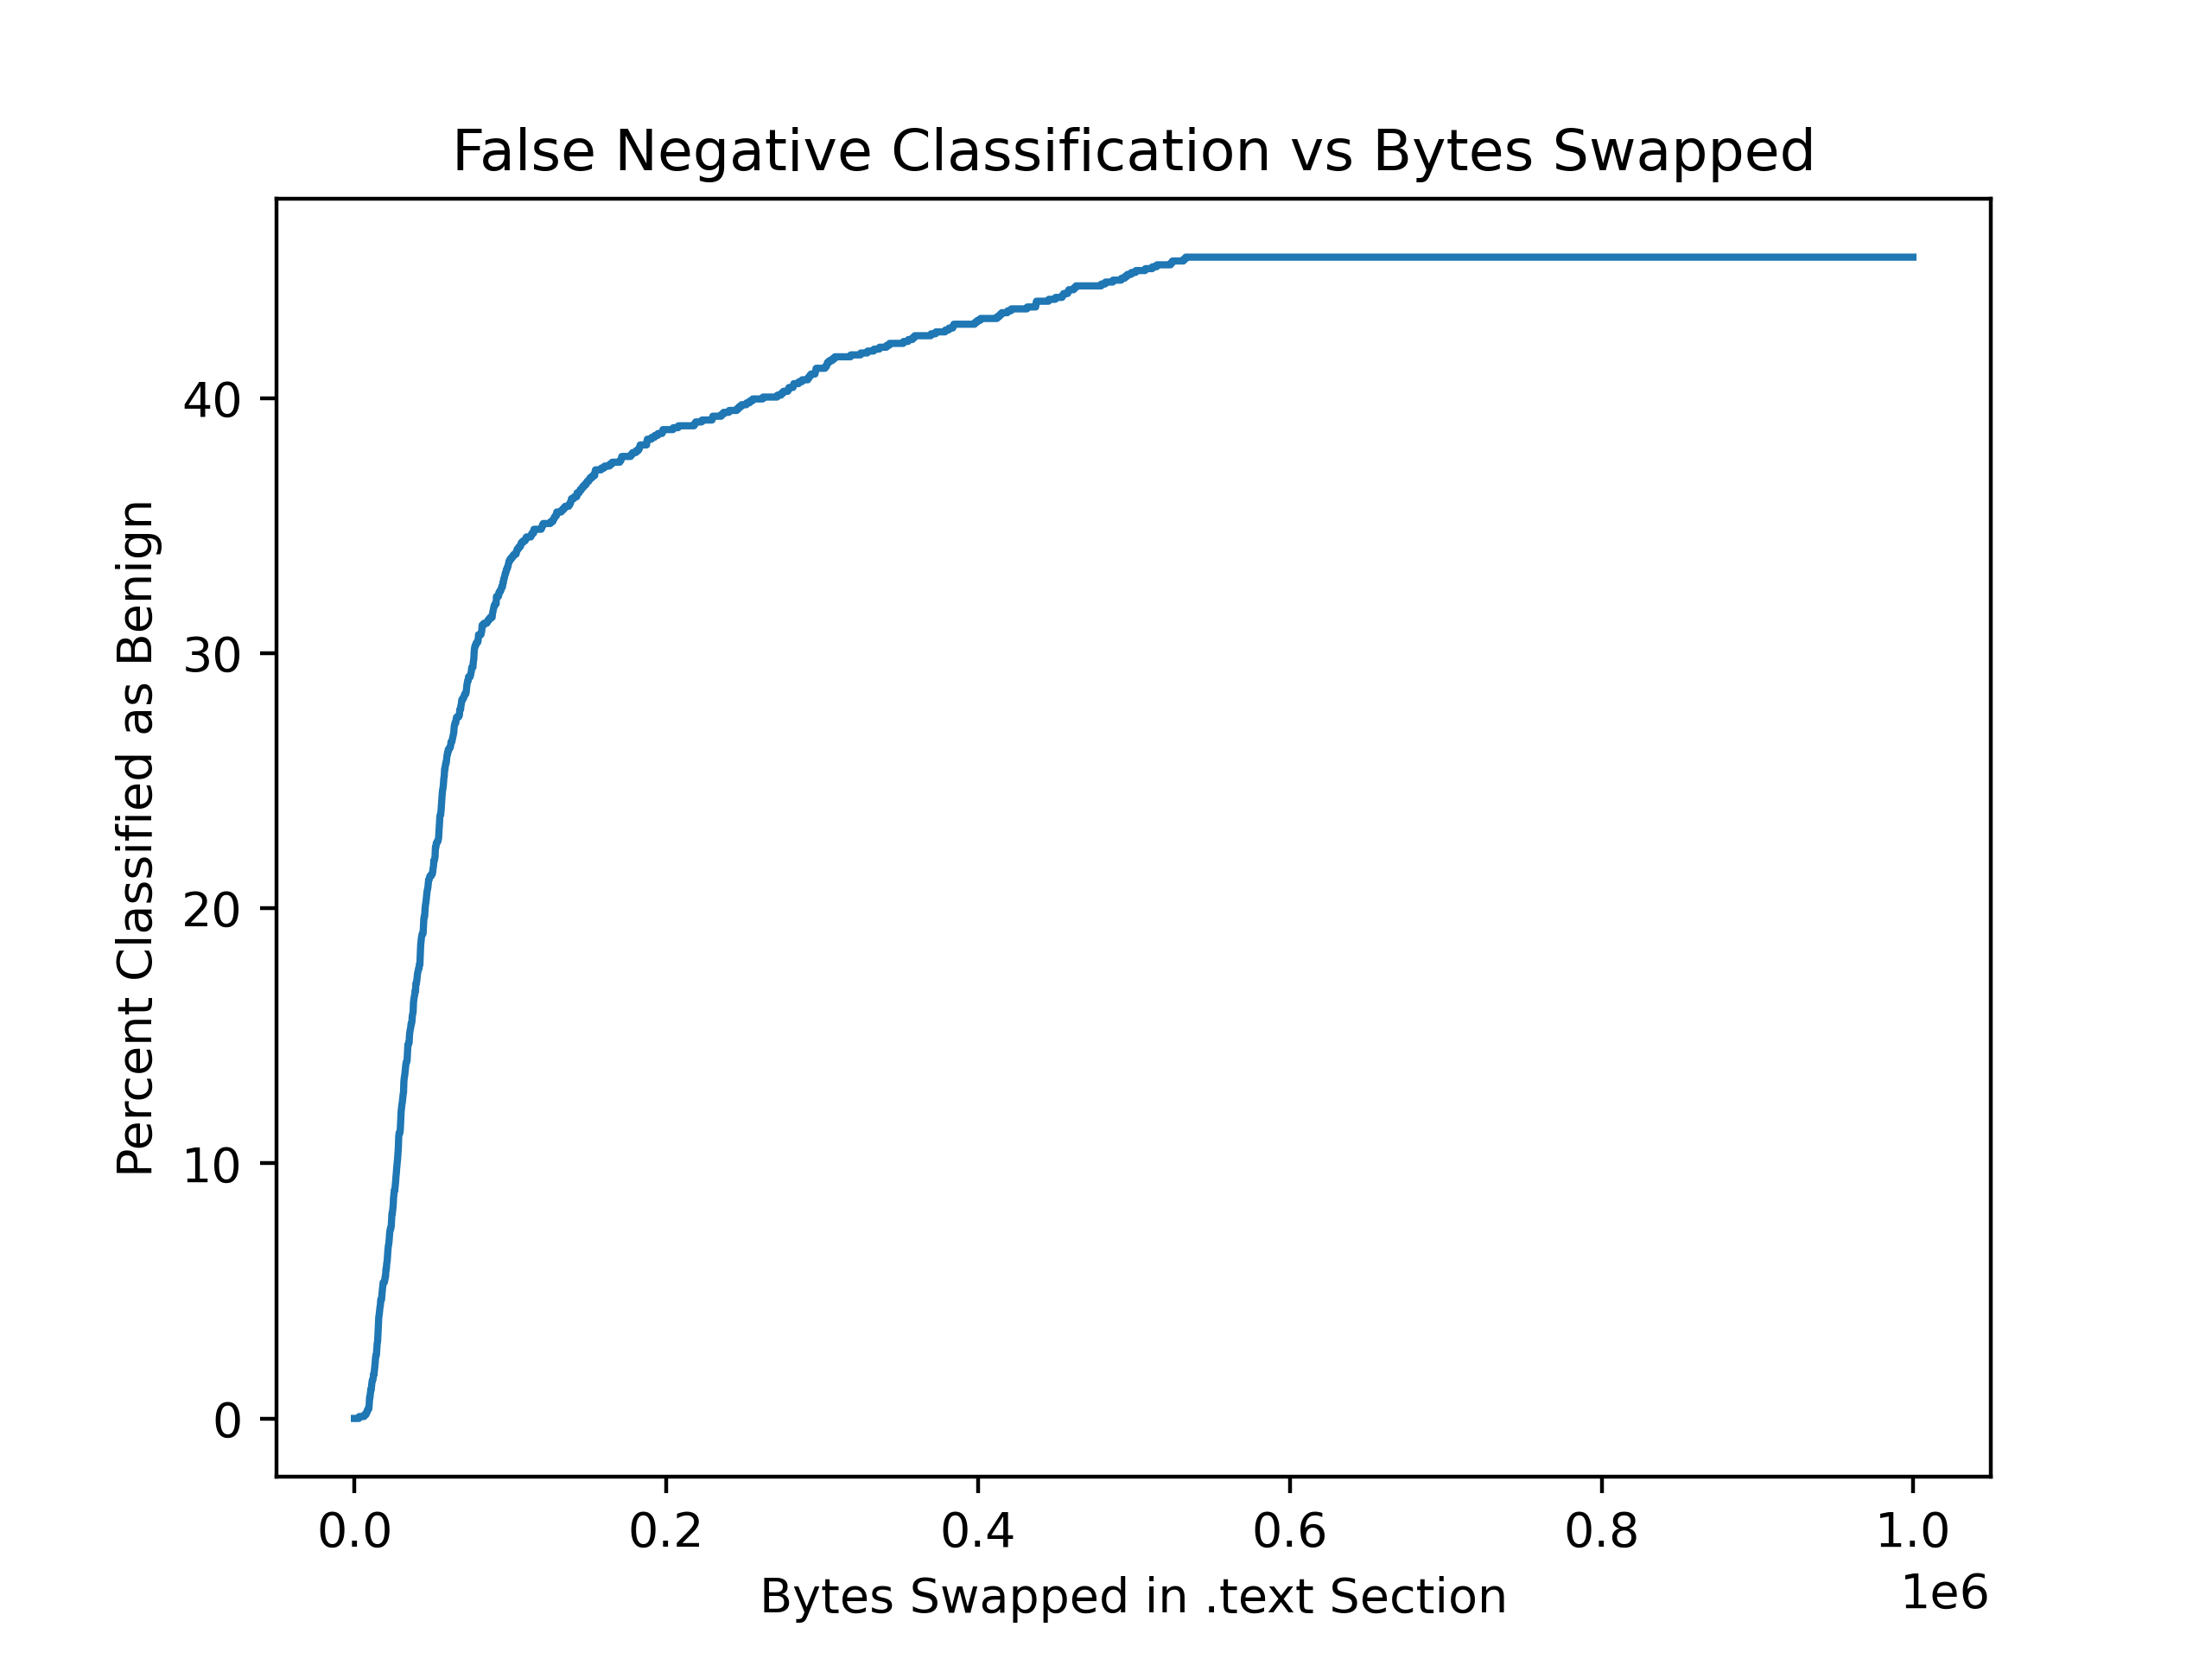
\includegraphics[scale=.5]{./figures/inc_benign/proportion_negative_vs_swap_absolute_any.png}
		\caption{Number of bytes swapped.}
	\end{subfigure}%
	\begin{subfigure}{.5\textwidth}
		\centering
		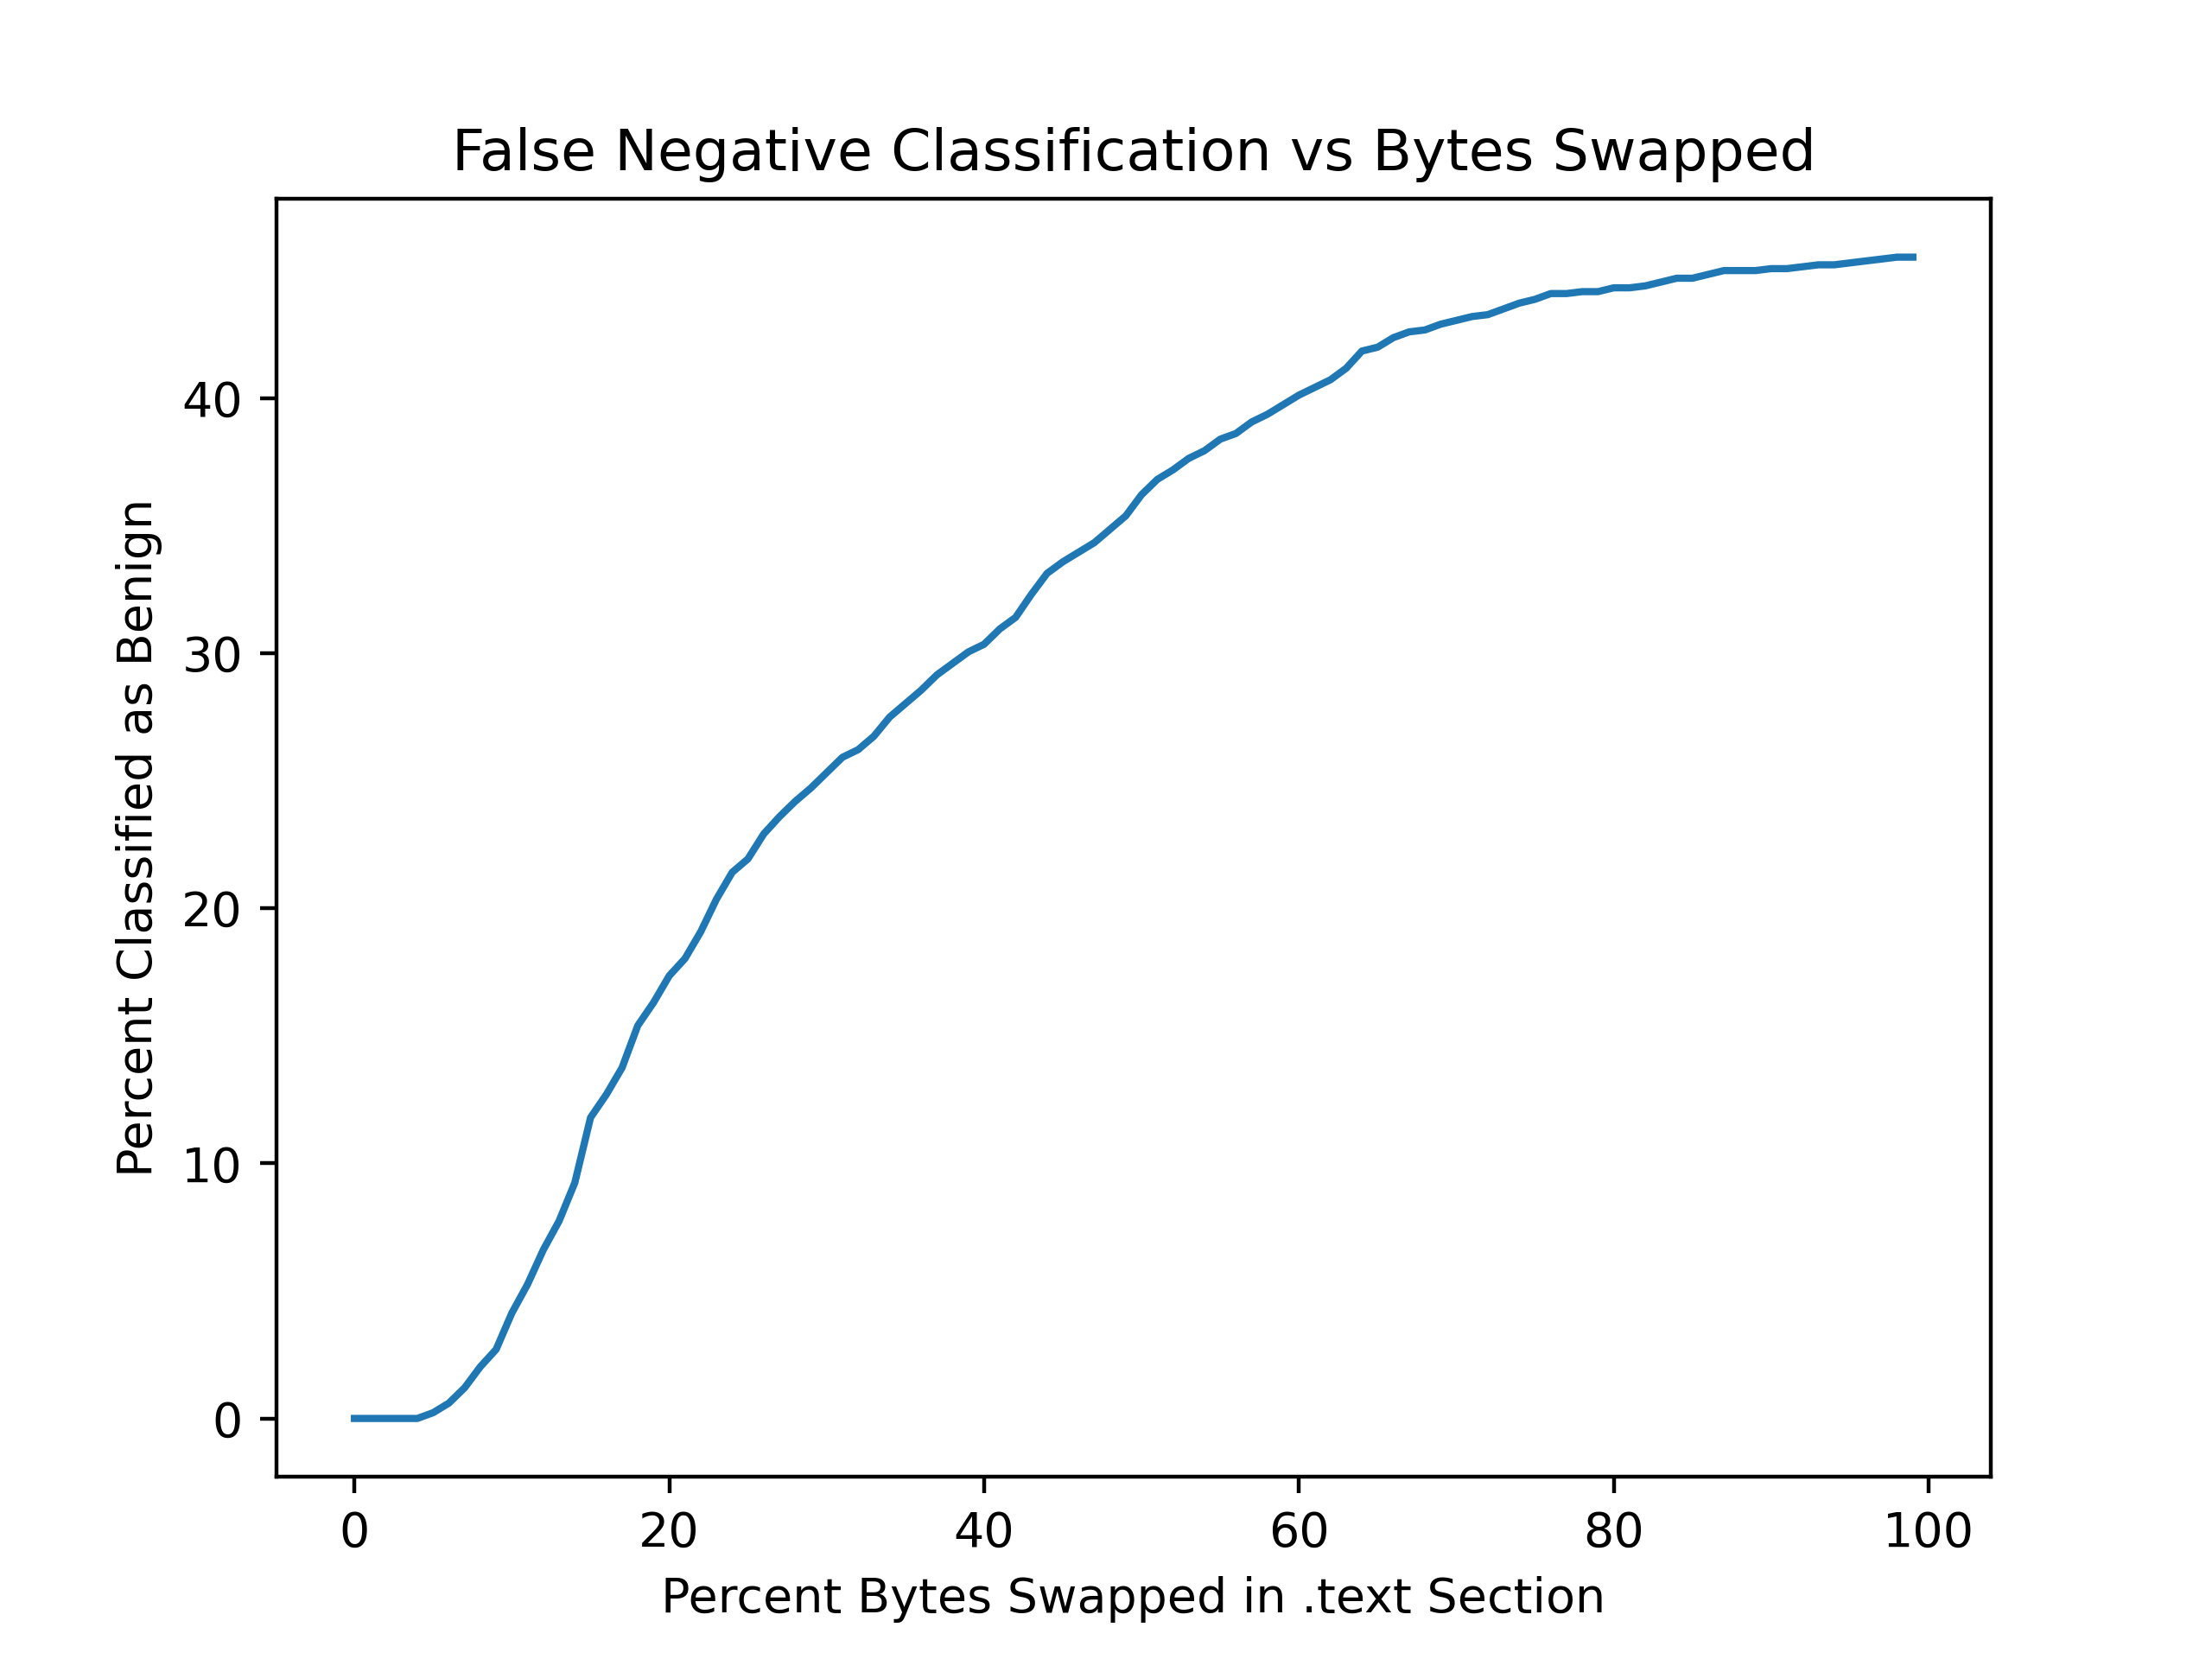
\includegraphics[scale=.5]{./figures/inc_benign/proportion_negative_vs_swap_proportion_any.png}
		\caption{Proportion of bytes swapped.}
	\end{subfigure}
	\caption{The false negative rate as more bytes from the .text section are replaced with bytes from a benign file. This is an average over 1500 malware files.}
\end{figure}

\noindent Analysis:
\begin{itemize}
	\item The left-hand figure is much sharper than the right-hand figure
	\item This is because the size of the .text sections of the malware files is severely skewed right (many malware files with small .text sections; few malware with large .text sections)
	\item These results indicate that a significant proportion of the bytes in the .text section would have to be altered to successfully evade a classifier
	\item However, results in the next section seem to indicate that higher evasion rates can be achieved if the replacement bytes are better selected
\end{itemize}

\subsubsection*{Full Swap}

Algorithm:
\begin{itemize}
	\item Identify the .text section of malware
	\item Replace entirely with bytes
	\begin{itemize}
		\item Random bytes - random values
		\item Padding byte - the padding byte value used by the classifier
		\item Benign bytes - the .text section from one of several different benign files. Benign files 0, 1, \& 2 are from the training set; benign files 3, 4, \& 5 are unseen by the classifier.
	\end{itemize}
	\item This is significantly faster than doing it incrementally, so I have a bit more flexibility in how I do things
	\item There are actually more malware files in this experiment and some of the files are an order of magnitude larger than the previous experiment, which is why some of the results are slightly different
	\item This classifier is unsurprisingly extremely over confident, see Figure 2
\end{itemize}

\begin{center}
	\begin{tabular}{| c | c |}
		\hline
		benign file & Confidence (\%) \\
		\hline 
		0 & 9.90 e-04  \% \\   
		1 & 3.37 e-04 \% \\   
		2 & 98.9 e-00     \% \\ 
		3 & 1.67 e-04 \% \\ 
		4 & 4.36 e-00  \% \\
		5 & 4.98 e-03  \% \\
		\hline
	\end{tabular}
\end{center}

\begin{center}
	\begin{tabular}{| c | c | c |}
		\hline
		method & Average difference in confidence (\%) & TP examples flipped to FP (\%) \\
		\hline 
		random & -0.35\% & 0\% \\  
		padding & -0.14\% & 0\% \\
		benign file 0 & -49\% & 48\% \\   
		benign file 1 & -68\% & 69\% \\   
		benign file 2 & -1.1\% & 0.76\% \\ 
		benign file 3 & -45\% & 43\% \\ 
		benign file 4 & -17\% & 13\% \\
		benign file 5 & -64\% & 63\% \\
		\hline
	\end{tabular}
\end{center}

\begin{figure}{h}
	\centering
	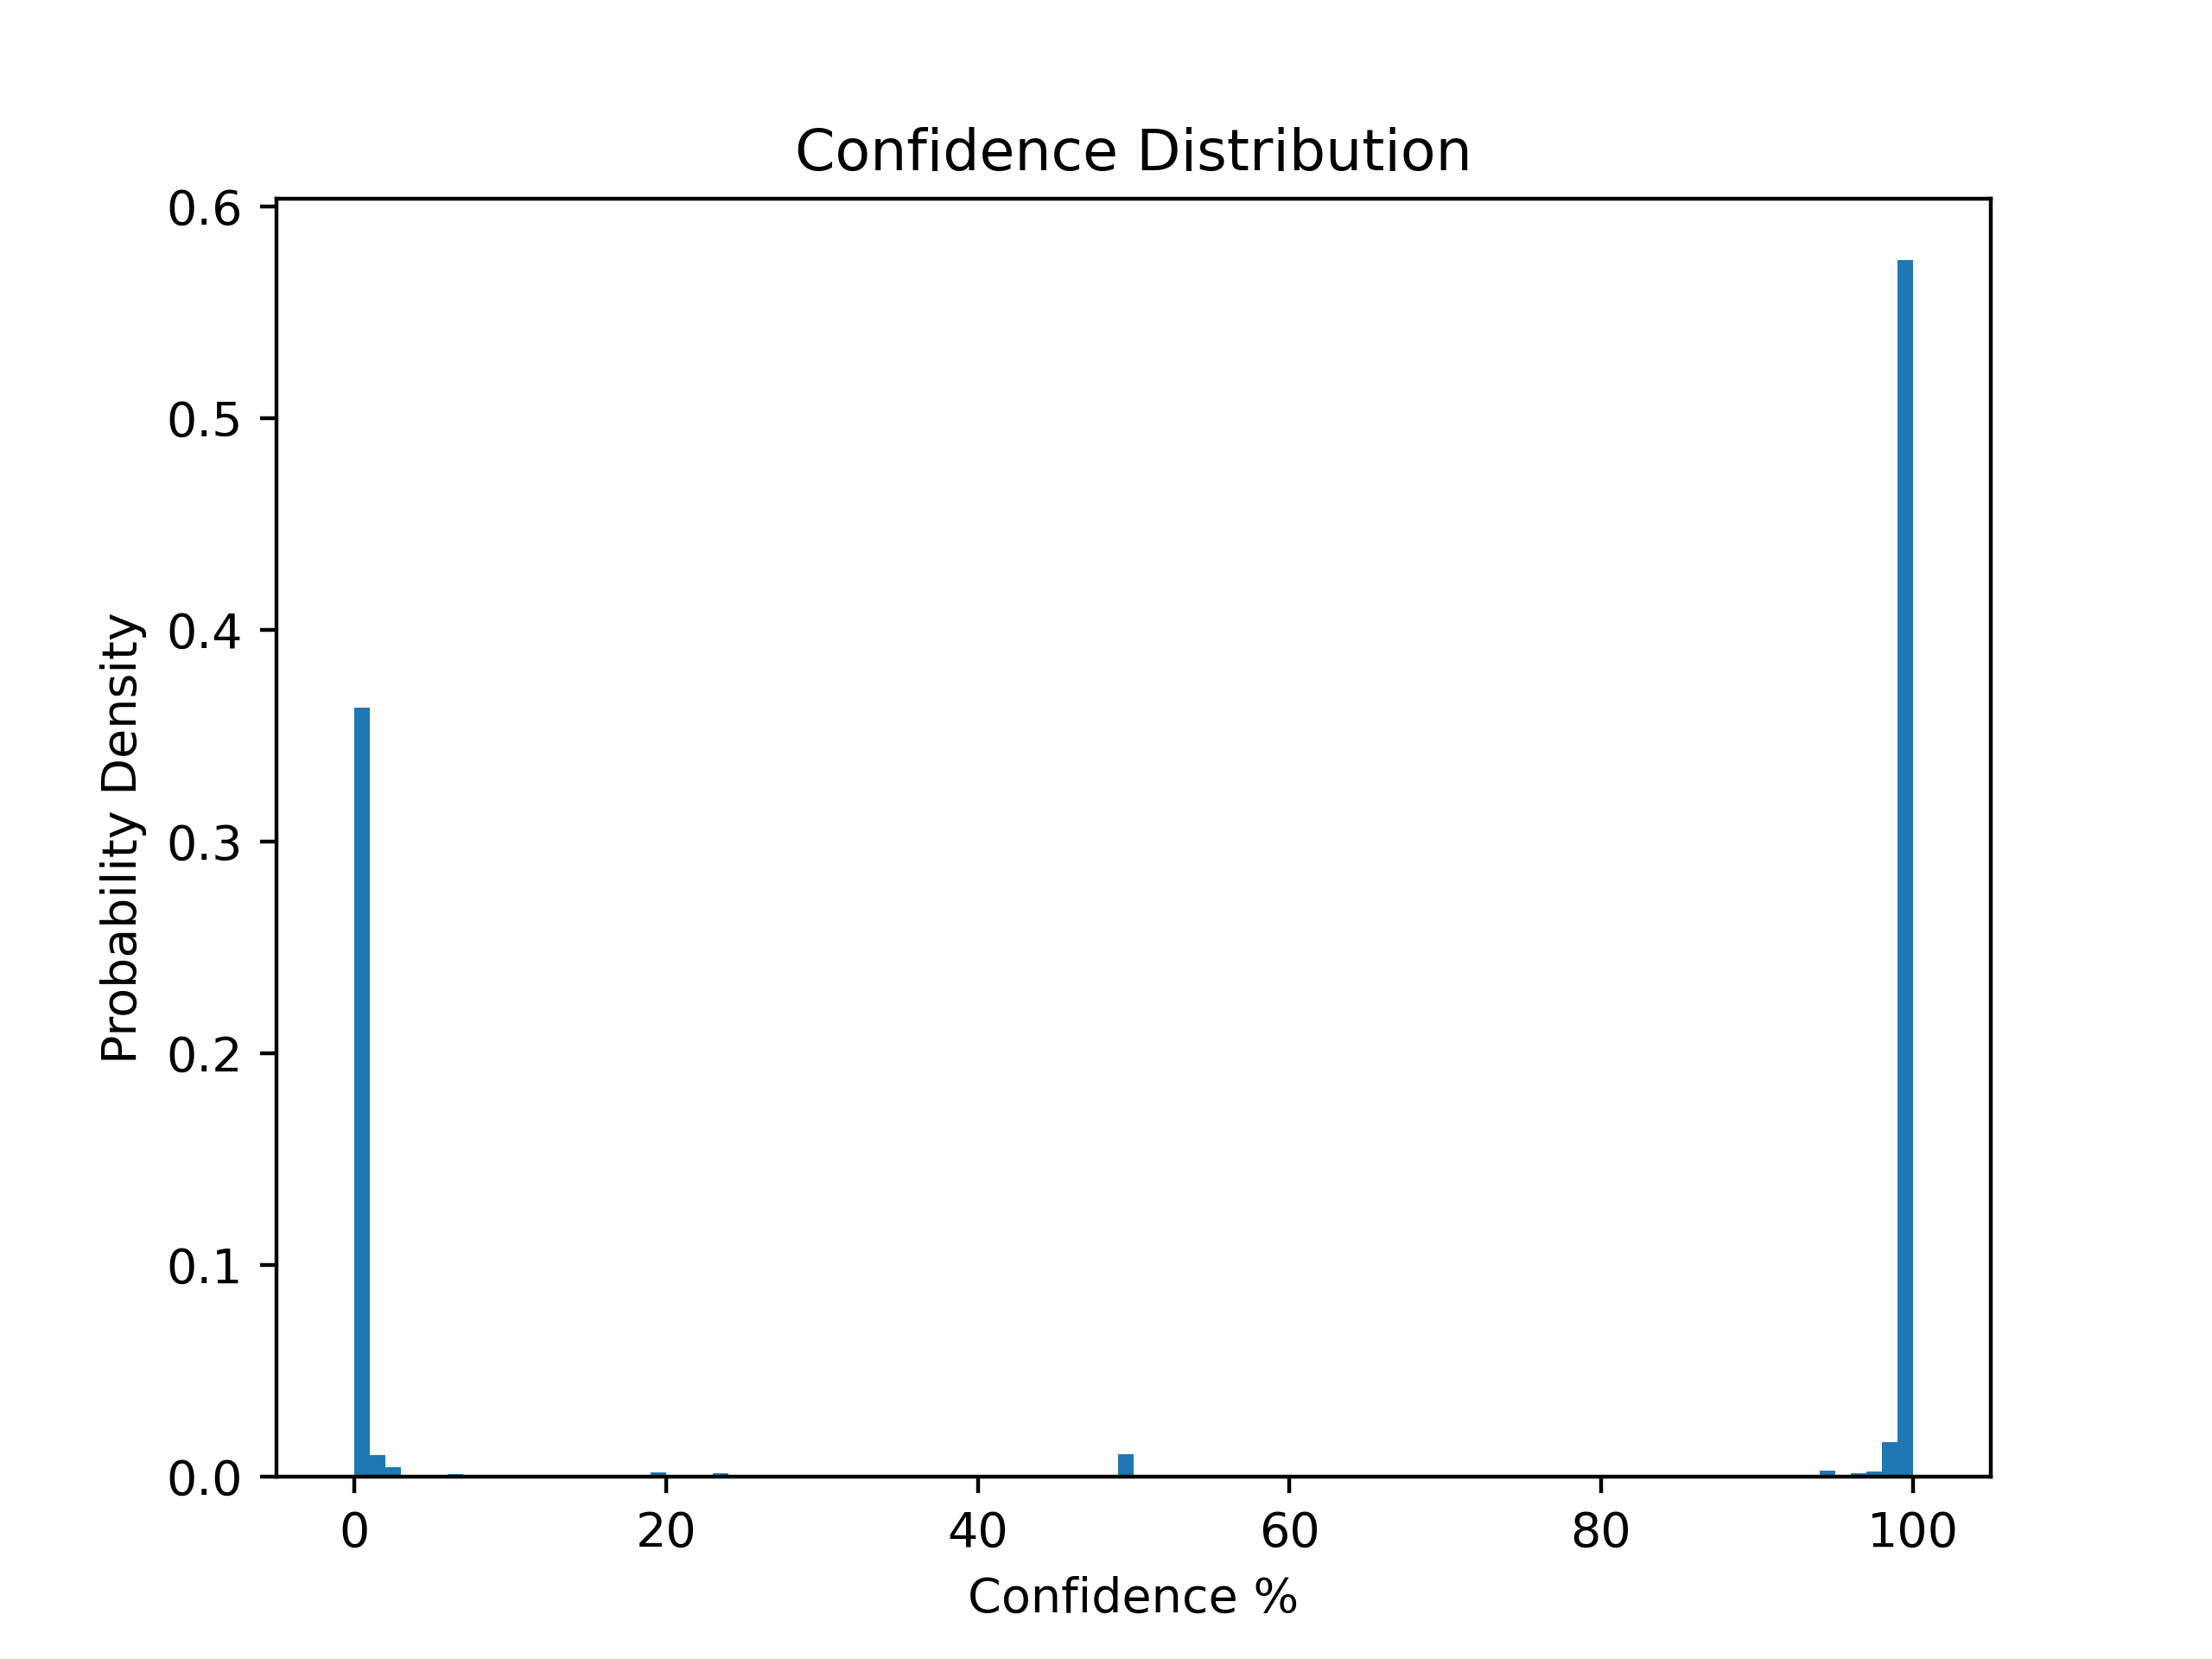
\includegraphics[scale=.5]{./figures/confidence_distribution.png}
	\caption{Distribution of confidence scores.}
\end{figure}

Analysis:
\begin{itemize}
	\item Replacing with random bytes or the padding byte was not effective
	\item Using different benign files as the swapping bytes can have a huge impact on the number of successful adversarial examples
\end{itemize}

\pagebreak

\section*{Week 13}
11:00 Monday 11/13/2022 - 10:59 Monday 11/20/2022

\subsection*{General}
\begin{itemize}
	\item CUDA\_VISIBLE\_DEVICES=2 python script.py
\end{itemize}

\subsection*{Report}
\begin{itemize}
	\item 
\end{itemize}

\subsection*{Minutes}
\begin{itemize}
	\item 
\end{itemize}

\pagebreak

\end{document}